%%%%%%%%%%%%%%%%%%%%%%%%%%%%%%%%%%%%%%%%%
% Lachaise Assignment
% LaTeX Template
% Version 1.0 (26/6/2018)
%
% This template originates from:
% http://www.LaTeXTemplates.com
%
% Authors:
% Marion Lachaise & François Févotte
% Vel (vel@LaTeXTemplates.com)
%
% License:
% CC BY-NC-SA 3.0 (http://creativecommons.org/licenses/by-nc-sa/3.0/)
%
%%%%%%%%%%%%%%%%%%%%%%%%%%%%%%%%%%%%%%%%%

%----------------------------------------------------------------------------------------
%	PACKAGES AND OTHER DOCUMENT CONFIGURATIONS
%----------------------------------------------------------------------------------------

\documentclass{article}

%%%%%%%%%%%%%%%%%%%%%%%%%%%%%%%%%%%%%%%%%
% Lachaise Assignment
% Structure Specification File
% Version 1.0 (26/6/2018)
%
% This template originates from:
% http://www.LaTeXTemplates.com
%
% Authors:
% Marion Lachaise & François Févotte
% Vel (vel@LaTeXTemplates.com)
%
% License:
% CC BY-NC-SA 3.0 (http://creativecommons.org/licenses/by-nc-sa/3.0/)
%
%%%%%%%%%%%%%%%%%%%%%%%%%%%%%%%%%%%%%%%%%

%----------------------------------------------------------------------------------------
%	PACKAGES AND OTHER DOCUMENT CONFIGURATIONS
%----------------------------------------------------------------------------------------

\usepackage{amsmath,amsfonts,stmaryrd,amssymb} % Math packages

\usepackage{enumerate} % Custom item numbers for enumerations

\usepackage[ruled]{algorithm2e} % Algorithms

\usepackage[framemethod=tikz]{mdframed} % Allows defining custom boxed/framed environments

\usepackage{listings} % File listings, with syntax highlighting

\usepackage{color} %red, green, blue, yellow, cyan, magenta, black, white
\definecolor{mygreen}{RGB}{28,172,0} % color values Red, Green, Blue
\definecolor{mylilas}{RGB}{170,55,241}
\usepackage{float}
\usepackage{amsmath}% http://ctan.org/pkg/amsmath
\newcommand\Inn{%
  \mathrel{\ooalign{$\subset$\cr\hfil\scalebox{0.8}[1]{$=$}\hfil\cr}}%
}
% \mathcode`*=\string"8000

\lstset{
	basicstyle=\ttfamily, % Typeset listings in monospace font
}


% matlab desciption
% usage \lstinputlisting{/path/to/matlab/code.m}

\lstset{language=Matlab,%
    %basicstyle=\color{red},
    breaklines=true,%
    morekeywords={matlab2tikz},
    keywordstyle=\color{blue},%
    morekeywords=[2]{1}, keywordstyle=[2]{\color{black}},
    identifierstyle=\color{black},%
    stringstyle=\color{mylilas},
    commentstyle=\color{mygreen},%
    showstringspaces=false,%without this there will be a symbol in the places where there is a space
    numbers=none,%
    numberstyle={\tiny \color{black}},% size of the numbers
    numbersep=9pt, % this defines how far the numbers are from the text
    emph=[1]{for,end,break},emphstyle=[1]\color{red}, %some words to emphasise
    %emph=[2]{word1,word2}, emphstyle=[2]{style},
}


%----------------------------------------------------------------------------------------
%	DOCUMENT MARGINS
%----------------------------------------------------------------------------------------

\usepackage{geometry} % Required for adjusting page dimensions and margins

\geometry{
	paper=a4paper, % Paper size, change to letterpaper for US letter size
	top=2.5cm, % Top margin
	bottom=3cm, % Bottom margin
	left=2.5cm, % Left margin
	right=2.5cm, % Right margin
	headheight=14pt, % Header height
	footskip=1.5cm, % Space from the bottom margin to the baseline of the footer
	headsep=1.2cm, % Space from the top margin to the baseline of the header
	%showframe, % Uncomment to show how the type block is set on the page
}

%----------------------------------------------------------------------------------------
%	FONTS
%----------------------------------------------------------------------------------------

\usepackage[utf8]{inputenc} % Required for inputting international characters
\usepackage[T1]{fontenc} % Output font encoding for international characters

\usepackage{XCharter} % Use the XCharter fonts

%----------------------------------------------------------------------------------------
%	COMMAND LINE ENVIRONMENT
%----------------------------------------------------------------------------------------

% Usage:
% \begin{commandline}
%	\begin{verbatim}
%		$ ls
%
%		Applications	Desktop	...
%	\end{verbatim}
% \end{commandline}

\mdfdefinestyle{commandline}{
	leftmargin=10pt,
	rightmargin=10pt,
	innerleftmargin=15pt,
	middlelinecolor=black!50!white,
	middlelinewidth=2pt,
	frametitlerule=false,
	backgroundcolor=black!5!white,
	frametitle={Command Line},
	frametitlefont={\normalfont\sffamily\color{white}\hspace{-1em}},
	frametitlebackgroundcolor=black!50!white,
	nobreak,
}

% Define a custom environment for command-line snapshots
\newenvironment{commandline}{
	\medskip
	\begin{mdframed}[style=commandline]
}{
	\end{mdframed}
	\medskip
}

%----------------------------------------------------------------------------------------
%	FILE CONTENTS ENVIRONMENT
%----------------------------------------------------------------------------------------

% Usage:
% \begin{file}[optional filename, defaults to "File"]
%	File contents, for example, with a listings environment
% \end{file}

\mdfdefinestyle{file}{
	innertopmargin=1.6\baselineskip,
	innerbottommargin=0.8\baselineskip,
	topline=false, bottomline=false,
	leftline=false, rightline=false,
	leftmargin=2cm,
	rightmargin=2cm,
	singleextra={%
		\draw[fill=black!10!white](P)++(0,-1.2em)rectangle(P-|O);
		\node[anchor=north west]
		at(P-|O){\ttfamily\mdfilename};
		%
		\def\l{3em}
		\draw(O-|P)++(-\l,0)--++(\l,\l)--(P)--(P-|O)--(O)--cycle;
		\draw(O-|P)++(-\l,0)--++(0,\l)--++(\l,0);
	},
	nobreak,
}

% Define a custom environment for file contents
\newenvironment{file}[1][File]{ % Set the default filename to "File"
	\medskip
	\newcommand{\mdfilename}{#1}
	\begin{mdframed}[style=file]
}{
	\end{mdframed}
	\medskip
}

%----------------------------------------------------------------------------------------
%	NUMBERED QUESTIONS ENVIRONMENT
%----------------------------------------------------------------------------------------

% Usage:
% \begin{question}[optional title]
%	Question contents
% \end{question}

\mdfdefinestyle{question}{
	innertopmargin=1.2\baselineskip,
	innerbottommargin=0.8\baselineskip,
	roundcorner=5pt,
	nobreak,
	singleextra={%
		\draw(P-|O)node[xshift=1em,anchor=west,fill=white,draw,rounded corners=5pt]{%
		Question \theQuestion\questionTitle};
	},
}

\newcounter{Question} % Stores the current question number that gets iterated with each new question

% Define a custom environment for numbered questions
\newenvironment{question}[1][\unskip]{
	\bigskip
	\stepcounter{Question}
	\newcommand{\questionTitle}{~#1}
	\begin{mdframed}[style=question]
}{
	\end{mdframed}
	\medskip
}

%----------------------------------------------------------------------------------------
%	WARNING TEXT ENVIRONMENT
%----------------------------------------------------------------------------------------

% Usage:
% \begin{warn}[optional title, defaults to "Warning:"]
%	Contents
% \end{warn}

\mdfdefinestyle{warning}{
	topline=false, bottomline=false,
	leftline=false, rightline=false,
	nobreak,
	singleextra={%
		\draw(P-|O)++(-0.5em,0)node(tmp1){};
		\draw(P-|O)++(0.5em,0)node(tmp2){};
		\fill[black,rotate around={45:(P-|O)}](tmp1)rectangle(tmp2);
		\node at(P-|O){\color{white}\scriptsize\bf !};
		\draw[very thick](P-|O)++(0,-1em)--(O);%--(O-|P);
	}
}

% Define a custom environment for warning text
\newenvironment{warn}[1][Warning:]{ % Set the default warning to "Warning:"
	\medskip
	\begin{mdframed}[style=warning]
		\noindent{\textbf{#1}}
}{
	\end{mdframed}
}

%----------------------------------------------------------------------------------------
%	INFORMATION ENVIRONMENT
%----------------------------------------------------------------------------------------

% Usage:
% \begin{info}[optional title, defaults to "Info:"]
% 	contents
% 	\end{info}

\mdfdefinestyle{info}{%
	topline=false, bottomline=false,
	leftline=false, rightline=false,
	nobreak,
	singleextra={%
		\fill[black](P-|O)circle[radius=0.4em];
		\node at(P-|O){\color{white}\scriptsize\bf i};
		\draw[very thick](P-|O)++(0,-0.8em)--(O);%--(O-|P);
	}
}

% Define a custom environment for information
\newenvironment{info}[1][Info:]{ % Set the default title to "Info:"
	\medskip
	\begin{mdframed}[style=info]
		\noindent{\textbf{#1}}
}{
	\end{mdframed}
}
 % Include the file specifying the document structure and custom commands
\usepackage{graphicx}


%----------------------------------------------------------------------------------------
%	ASSIGNMENT INFORMATION
%----------------------------------------------------------------------------------------

\title{ENGR 8103: Problem Set \#5} % Title of the assignment

\author{Allen Spain\\ \texttt{avs81684@uga.edu}} % Author name and email address

\date{University of Georgia --- 10 October 2019 } % University, school and/or department name(s) and a date

%----------------------------------------------------------------------------------------

\begin{document}

\maketitle % Print the title

%----------------------------------------------------------------------------------------
%	INTRODUCTION
%----------------------------------------------------------------------------------------


\section*{Problem 1} % Unnumbered section
If $T = A(h) + a_{1} h^{1/2} + a_{2} h^{2/2} + a_{3} h^{3/2},$ then what combination of $A(h)$ and $A(h/2)$ should give an accurate estimate of $T$ ?

\begin{equation}
T = A(h) + a_{1}h^{1/2} + a_{2}h^{2/2} + a_{3}h^{3/2}  + \cdots\\
\end{equation}

\begin{equation}
T = A(h/2) + \frac{a_{1}h^{1/2}}{2^{1/2}} + \frac{a_{2}h^{1}}{2} +\\ \frac{a_{3}h^{3/2}}{2^{3/2}} + \cdots
\end{equation}

Combine (1) and equation (2) as follows $T - \frac{-T}{\sqrt{2}} $ this yields the resultant equation:

\begin{equation}
T - \frac{T}{\sqrt{2}} =  A(h/2) - \frac{A(h)}{\sqrt{2}} + \underbrace{ \frac{a_{2}h^{1}}{2} + \frac{a_{3}h^{3/2}}{2^3/2} - \frac{a_{3}h^{3/2}}{\sqrt{2}} + \cdots}_\text{Error (E)}
\end{equation}

Therefore the combination of $A(h) and A(h/2)$ is as follows:

\begin{equation}
T = \frac{A(h/2) - \frac{A(h)}{\sqrt{2}}}{1-\frac{1}{\sqrt{2}}} + E
\end{equation}



\section*{Problem 2} % Unnumbered section
Consider a second order approximation $A(h)$ to $T$ such that
\begin{equation}
T = A(h) + a_{2}h^{2} + a_{4}h^{4} + a_{6}h^{6} + \cdots
\end{equation}

a) Find a sixth order approximation to $T$ using $A(h), A(2h), A(3h)$

Using step size $ 2h $

\begin{equation}
-T = A(2h) + 4a_{2}h^{2} + 16a_4h^{4} + 32a_{6}h^{6} + \cdots
\end{equation}

Combining equation 5 and 6.
\begin{equation}
-T = A(2h) + 4a_{2}h^{2} + 16a_4h^{4} + 32a_{6}h^{6} + \cdots \\
\end{equation}

\begin{equation}
	4T = 4A(h) + 4a_{2}h^{2} + 4a_{4}h^{4} + 4a_{6}h^{6} + \cdots \\
\end{equation}

\begin{equation}
	 \approx 3T = 4A(h) - A(2h) - 12a_{4}h^{4} - \frac{60a_{6}}{h^{6}}{3} \cdots \\
\end{equation}

\begin{equation}
  T = \dfrac{4A(h) - A(2h)}{3} - 4a_{4}h^{4} - 20a_{6}h^{6} + \cdots
\end{equation}

Now coarse correction using step size $3h$

\begin{equation}
  T = A(3h) + 9a_{2}h^{2} + 81a_{4}h^{4} + 729a_{6}h^{6} + \cdots
\end{equation}

Combining equation 12 and 5
\begin{equation}
 9T = 9A(h) + 9a_{2}h^{2} + 9a_{4}h^{4} + 9a_{6}h^{6} + \cdots
\end{equation}

\begin{equation}
-T = A(3h) + 9a_{2}h^{2} + 81a_{4}h^{4} + 729a_{6}h^{6} + \cdots
\end{equation}

\begin{equation}
\approx 9T - T = 9A(h) - A(3h) - 72a_{4}h^{4} - 720a_{6}h^{6} + \cdots
\end{equation}

This yields...
\begin{equation}
T = \frac{9A(h) - A(3h)}{8} - 9a_{4}h^{4} - 90a_{6}h^{6} + \cdots
\end{equation}

Cancel out high order term using equation 8 and equation 15
\begin{equation}
(4T = 4A(h) + 4a_{2}h^{2} + 4a_{4}h^{4} + 4a_{6}h^{6} + \cdots) * 9
\end{equation}

\begin{equation}
(T = \frac{9A(h) - A(3h)}{8} - 9a_{4}h^{4} - 90a_{6}h^{6} + \cdots) * -4
\end{equation}

Subtract the equations
\begin{equation}
5T = \frac{3A(h)}{2} - \frac{3A(2h)}{5} - \frac{A(3h)}{10} + 180a_{6}h^{6}
\end{equation}

Solving gives you a 6th approximation of of $T$
\begin{equation}
T = \frac{3A(h)}{2} - \frac{3A(2h)}{5} - \frac{A(3h)}{10} + 180a_{6}h^{6}
\end{equation}

b) Applying part a)
\begin{equation}
T = \underbrace{\frac{3A(h)}{2} - \frac{3A(2h)}{5} - \frac{A(3h)}{10} + 180a_{6}h^{6} + \cdots}_\text{A(h)}
\end{equation}


\begin{equation}
A(h) = \frac{1}{h^2}[f(x+h) -2f(x) + f(x-h)] + \mathcal{O}(h^{6})
\end{equation}

By finding the common denominator of all of the fractional componenents in equation 20 you can solve the following
\begin{equation}
f''(x) = \frac{1}{36h^{2}}[ 49f(x+h)+ 49f(x+2h) + 49 f(x + 3h) - 294f(x) + 49f(x - h) + 49f(x -2h) + 49f(x -3h)] + \mathcal{O}(h^{6})
\end{equation}


\section*{Problem 3} % Unnumbered section

\noindent
(a): Consider the following IVP ?
% Math equation/formula
\begin{equation}
	x ^{\prime} = 1 + t + x^2
\end{equation}

\begin{equation}
  x(0) = 1
\end{equation}

\lstinputlisting{/Users/allenspain/Documents/Development/MATLAB/comp-engr/hw5/euler.m}

\begin{verbatim}
-------------------

Ouput:

index:0 1
index:1 3
index:2 14
index:3 213
index:4 45586

-------------------
\end{verbatim}

\begin{figure}
  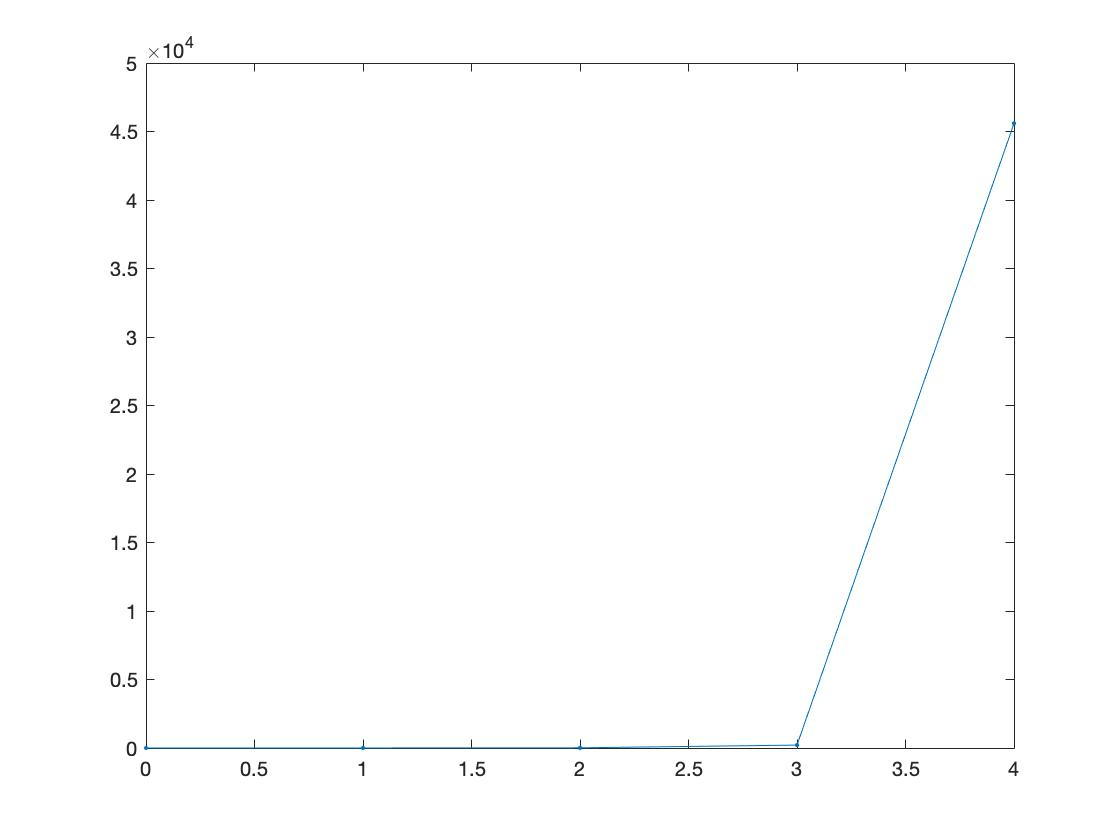
\includegraphics[width=\linewidth]{docs/euler.jpg}
  \caption{Euler's method for approximating $x$}
  \label{fig:boat1}
\end{figure}

From Euler's method $ x(2) = 14$ \\


(b): Use second-order Taylor Series method to estimate $x(2)$ with step size $h = 1$

\lstinputlisting{/Users/allenspain/Documents/Development/MATLAB/comp-engr/hw5/taylor_series.m}

\begin{verbatim}
-------------------
Ouput:

index:0 1
index:1 5.500000e+00
index:2 2.156250e+02
index:3 1.007266e+07
index:4 1.021957e+21

-------------------
\end{verbatim}

\noindent
Using Taylor series second order approximation $x(2) \approx 215$\\


\noindent

(c): Use third-order Taylor Series method to estimate $x(2)$ with step size  $ h = 1$ \\
$ x(2) \approx  399410 $

\lstinputlisting{/Users/allenspain/Documents/Development/MATLAB/comp-engr/hw5/taylor_series3.m}


\begin{verbatim}
-------------------
Ouput:

index:0 1
index:1 3
index:2 14
index:3 213
index:4 45586

-------------------
\end{verbatim}



\end{document}
